\taskpic{ На массивном бревне радиуса $R$ лежит лёгкий стержень длины $2L$, на
  обоих концах которого закреплены одинаковые камни массы
  $m$. Стержень выводят из равновесия слегка наклоняя один конец
  вниз. Найдите период колебаний стержня $T$. }
{
  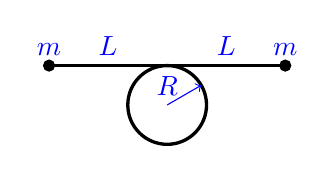
\begin{tikzpicture}
    \draw[very thick] (2,0.5) circle (0.5cm);
    \draw[very thick] (0.5,1) -- (3.5,1);
    \draw[fill=black] (0.5,1) circle (0.07cm) node[above,blue] {$m$};
    \draw[fill=black] (3.5,1) circle (0.07cm) node[above,blue] {$m$};
    \draw[blue,->] (2,0.5) node[above] {$R$} -- ++(30:0.5);
    \draw (1.25,1) node[blue,above] {$L$};
    \draw (2.75,1) node[blue,above] {$L$};
  \end{tikzpicture}
}
